\documentclass[a4paper,11pt]{report}
\author{Adrien Leman; Nicolas Bellot}
\title{Documentation of the project FA$\mu$ST \smallbreak "Flexible Approximate Multi-Layer Sparse Transform" \bigbreak
\bigbreak
\centerline{
\includegraphics[scale=0.1]{images/logo.png}}
}

\usepackage[]{mcode} % import matlab file
\usepackage[utf8]{inputenc}
\usepackage[T1]{fontenc}
\usepackage[margin=1in]{geometry}
\usepackage{graphicx, subcaption, enumerate}
\usepackage{amsmath}
\usepackage{amsfonts}
%\usepackage{amsthm}
\usepackage[boxruled,algo2e]{algorithm2e}

%\newcommand\mycommfont[1]{\footnotesize\ttfamily\textcolor{blue}{#1}}
%\newcommand\mPAT[1]{\marginpar{\footnotesize\textcolor{blue}{PP:~#1}}}
%\newcommand\PAT[1]{\textcolor{blue}{#1}}
%\newcommand\mRG[1]{\marginpar{\footnotesize\textcolor{blue}{RG:~#1}}}
%\newcommand\RG[1]{\textcolor{blue}{#1}}
%\newcommand\todoRG[1]{\textcolor{red}{RG:~#1}}
%\newcommand\todoPP[1]{\textcolor{red}{PP:~#1}}
%\definecolor{darkgreen}{rgb}{0,0.8,0}
%\newcommand\mNK[1]{\marginpar{\footnotesize\textcolor{blue}{NK:~#1}}}
%\newcommand\NK[1]{\textcolor{ForestGreen}{#1}}
%\newcommand\todoNK[1]{\textcolor{red}{NK:~#1}}
\SetCommentSty{mycommfont}

\usepackage{algorithmic}
\usepackage{comment}
\usepackage[dvipsnames]{xcolor}
\usepackage{enumitem}
\usepackage{url}
\usepackage{multirow}
\usepackage{sectsty}
\usepackage[font=small,labelfont=bf]{caption}
\usepackage{placeins}
\usepackage{epstopdf}
\usepackage{hyperref}
\usepackage{tikz}
%\usepackage{appendix}
\usepackage{mathtools}
\usepackage[]{listings}
\definecolor{mygreen}{rgb}{0,0.6,0}
\definecolor{mygray}{rgb}{0.95,0.95,1}
\definecolor{mymauve}{rgb}{0.58,0,0.82}
\lstset{ %
  backgroundcolor=\color{mygray},   % choose the background color; you must add \usepackage{color} or \usepackage{xcolor}
  basicstyle=\ttfamily,        % the size of the fonts that are used for the code
%  breakatwhitespace=false,         % sets if automatic breaks should only happen at whitespace
  breaklines=true,                 % sets automatic line breaking
%  captionpos=b,                    % sets the caption-position to bottom
  commentstyle=\color{mygreen},    % comment style
%  deletekeywords={...},            % if you want to delete keywords from the given language
%  escapeinside={\%*}{*)},          % if you want to add LaTeX within your code
  extendedchars=true,              % lets you use non-ASCII characters; for 8-bits encodings only, does not work with UTF-8
  frame=single,	                   % adds a frame around the code
  keepspaces=true,                 % keeps spaces in text, useful for keeping indentation of code (possibly needs columns=flexible)
%  keywordstyle=\color{blue},       % keyword style
  language=Octave,                 % the language of the code
%  otherkeywords={*,...},           % if you want to add more keywords to the set
  numbers=left,                    % where to put the line-numbers; possible values are (none, left, right)
  numbersep=5pt,                   % how far the line-numbers are from the code
  numberstyle=\tiny\color{gray}, % the style that is used for the line-numbers
  rulecolor=\color{black},         % if not set, the frame-color may be changed on line-breaks within not-black text (e.g. comments (green here))
%  showspaces=false,                % show spaces everywhere adding particular underscores; it overrides 'showstringspaces'
%  showstringspaces=false,          % underline spaces within strings only
%  showtabs=false,                  % show tabs within strings adding particular underscores
%  stepnumber=2,                    % the step between two line-numbers. If it's 1, each line will be numbered
  stringstyle=\color{mymauve},     % string literal style
%  tabsize=2,	                   % sets default tabsize to 2 spaces
%  title=\lstname                   % show the filename of files included with \lstinputlisting; also try caption instead of title
}

% bold symbols
\newcommand{\bfA}{\mathbf{A}}
\newcommand{\bfX}{\mathbf{X}}
\newcommand{\bfW}{\mathbf{W}}
\newcommand{\bfD}{\mathbf{D}}
\newcommand{\bfQ}{\mathbf{Q}}
\newcommand{\bfR}{\mathbf{R}}
\newcommand{\bfM}{\mathbf{M}}
\newcommand{\bfw}{\mathbf{w}}
\newcommand{\bfz}{\mathbf{z}}
\newcommand{\bfx}{\mathbf{x}}
\newcommand{\bfr}{\mathbf{r}}
\newcommand{\bfe}{\mathbf{e}}
\newcommand{\bfy}{\mathbf{y}}
\newcommand{\hbfz}{\hat{\mathbf{z}}}
\newcommand{\bfI}{\mathbf{I}}
\newcommand{\bfU}{\mathbf{U}}
\newcommand{\bfu}{\mathbf{u}}
\newcommand{\bfV}{\mathbf{V}}
\newcommand{\bfv}{\mathbf{v}}


% sums
\newcommand{\sump}{\sum_{p=1}^P}
\newcommand{\summ}{\sum_{j=1}^m}
\newcommand{\sumk}{\sum_{k=1}^K}
\newcommand{\sumt}{\sum_{t=1}^T}
\newcommand{\sumko}{\sum_{k_1=1}^K}
\newcommand{\sumkt}{\sum_{k_2=1}^K}
\newcommand{\sumn}{\sum_{i=1}^N}


% general
\newcommand{\dataset}{\mathcal{X}}
\newcommand{\fhalf}{\frac{1}{2}}
\newcommand{\neucl}[1]{\left\lVert#1\right\rVert_2}
\newcommand{\ipeucl}[2]{\left\langle #1,#2 \right\rangle_2}
\newcommand{\smeas}{\mathcal{M}}
\newcommand{\pmeas}{\mathcal{P}}
\newcommand{\gaussset}{\mathcal{G}}
\newcommand{\gaussmix}[1]{{\mathcal{G}_{#1}}}
\newcommand{\sph}[1]{\mathcal{S}_{#1-1}}
\newcommand{\fracsqm}{\frac{1}{\sqrt{m}}}
\newcommand{\sqm}{\sqrt{m}}
\newcommand{\argmin}[1]{\underset{#1}{\text{argmin}}}


% sketches
\newcommand{\freqs}{\Omega} %frequencies
\newcommand{\freq}{{\boldsymbol\omega}} %frequency
\newcommand{\scalfreq}{\omega}
\newcommand{\hyppar}{\Theta} %hyper parameter
\newcommand{\chrc}{\psi} %characteristic function
\newcommand{\skop}{\mathcal{A}} %sketching operator
\newcommand{\malpha}{{\boldsymbol\alpha}} %weights (to rename)
\newcommand{\mmu}{{\boldsymbol\mu}} %means
\newcommand{\mSigma}{{\boldsymbol\Sigma}} %variances
\newcommand{\msigma}{{\boldsymbol\sigma}} %diag variances
\newcommand{\mrho}{{\boldsymbol\varphi}} %frequency angle
\newcommand{\mtheta}{{\boldsymbol\theta}} %frequency radius
\newcommand{\relsprs}{\rho} %relative sparsity (for results)
\newcommand{\relmsrm}{\delta} %relative number of parameters (for results)
\newcommand{\thetaset}{\mathcal{T}}
%\newcommand{\thetaset}{\Theta}
\newcommand{\Nsmall}{{N_{small}}}
\newcommand{\msmall}{{m_{small}}}
\newcommand{\gmmcover}{\Gamma}
\newcommand{\pp}{P}
\newcommand{\PP}{\mathbb{P}}
\newcommand{\qq}{Q}
\newcommand{\dens}{p}
\newcommand{\cstdom}{\mathrm{A}}

% rkhs
\newcommand{\rkhs}{\mathcal{H}}
\newcommand{\ipH}[2]{\left\langle #1,#2 \right\rangle_\rkhs}
\newcommand{\normH}[2]{\gamma_k\left(#1,#2\right)}
\newcommand{\normHnota}{\gamma_k}
\newcommand{\featm}{\phi}
\newcommand{\freqdist}{\Lambda}
\newcommand{\freqdistn}{\hat{\Lambda}}
\newcommand{\model}{\Sigma}
\newcommand{\Xspace}{X}
\newcommand{\TIk}{\mathbf{K}}
\newcommand{\supp}{\text{\upshape supp}}
\newcommand{\secant}{\mathcal{S}}
\newcommand{\decod}{\Delta}
\newcommand{\enet}{\mathcal{N}}
\newcommand{\kernel}{\kappa}
\newcommand{\meas}{\nu} % to avoid mu, which is the mean of gaussian
\newcommand{\mmap}{\varphi}
\newcommand{\sigmaker}{\sigma_\freqdist}
\newcommand{\sigkersmall}{S}

%imaginary unit
\newcommand{\imaginaryi}{\mathsf{i}}

% misc
\definecolor{light-gray}{gray}{0.3}
\newcommand{\mycomment}[1]{\emph{\small \color{red} NK: #1}}
\newcommand{\mytodo}[1]{\emph{\color{blue} #1}}

% io proba
\newcommand{\bigprbsp}{\mathbf{S}}
\newcommand{\event}{E}
\newcommand{\eventset}{\mathcal{F}}
\newcommand{\prbfc}{\mathbb{P}}
\newcommand{\measop}{\mathbf{M}}
\newcommand{\eps}{\epsilon}
\newcommand{\outc}{s}
\newcommand{\decop}{\mathbf{y}'}
\newcommand{\skopprb}{\skop^{(\outc)}}
\newcommand{\pprb}{\hat{\pp}^{(\outc)}}
\newcommand{\pproj}{\pp_\text{proj}}

\newcommand{\distfun}[3]{\gamma_{#3}\left(#1,#2\right)}
\newcommand{\distfunsq}[3]{\gamma^2_{#3}\left(#1,#2\right)}
\newcommand{\distfuns}[1]{\gamma_{#1}}
\newcommand{\normE}[2]{\distfun{#1}{#2}{E}}
\newcommand{\normEs}{\distfuns{E}}
\newcommand{\normF}[2]{\distfun{#1}{#2}{F}}
\newcommand{\normFs}{\distfuns{F}}
\newcommand{\normX}[2]{\distfun{#1}{#2}{X}}
\newcommand{\normXs}{\distfuns{X}}
\newcommand{\normM}[2]{\distfun{#1}{#2}{M}}
\newcommand{\normMs}{\distfuns{M}}
\newcommand{\normG}[2]{\distfun{#1}{#2}{G}}
\newcommand{\normGs}{\distfuns{G}}
\newcommand{\normmix}[2]{\distfun{#1}{#2}{mix}}
\newcommand{\normmixs}{\distfuns{mix}}
\newcommand{\normK}[2]{\distfun{#1}{#2}{\freqdist}}
\newcommand{\normKs}{\distfuns{\freqdist}}
\newcommand{\normKsq}[2]{\distfunsq{#1}{#2}{\freqdist}}
\newcommand{\normker}[2]{\distfun{#1}{#2}{\kernel}}
\newcommand{\normkers}{\distfuns{\kernel}}
\newcommand{\normkersq}[2]{\distfunsq{#1}{#2}{\kernel}}

\newcommand{\diam}[1]{\text{\upshape diam}\left(#1\right)}
\newcommand{\rad}[1]{\text{\upshape radius}\left(#1\right)}

%\newcommand{\LRIPsu}{\text{LRIP}}
%\newcommand{\BPnu}{\text{BP}}
%\newcommand{\CIOPsu}{\text{CIOP}}
%\newcommand{\prop}{\Pi}
%\newcommand{\nSig}[2]{\|#1\|_{\sigma_{#2}^2}}
%\newcommand{\ipW}[2]{\left\langle #1,#2 \right\rangle_2}

\newcommand{\embd}{\phi}

\makeatletter
\newcommand{\nosemic}{\renewcommand{\@endalgocfline}{\relax}}% Drop semi-colon ;
\newcommand{\dosemic}{\renewcommand{\@endalgocfline}{\algocf@endline}}% Reinstate semi-colon ;
\newcommand{\pushline}{\Indp}% Indent
\newcommand{\popline}{\Indm\dosemic}% Undent
\makeatother

\newcommand{\code}[1]{\texttt{#1}}



\begin{document}

\maketitle

\tableofcontents
\newpage


\chapter{Introduction}\label{sec:intro}

\paragraph{Presentation:}FA$\mu$ST is a C++ toolbox, useful to decompose a given dense matrix into a product of sparse matrices in order to reduce its computational complexity (both for storage and manipulation). In Figure \ref{fig:presentation}, the matrix \textbf{A} represents the dense matrix and $\mathbf{S_j}$ correspond to the sparse matrices as $\mathbf{A}=\prod_{j=1}^J\mathbf{S_j}$.

\begin{figure}[H] %%[!htbp]
\centering
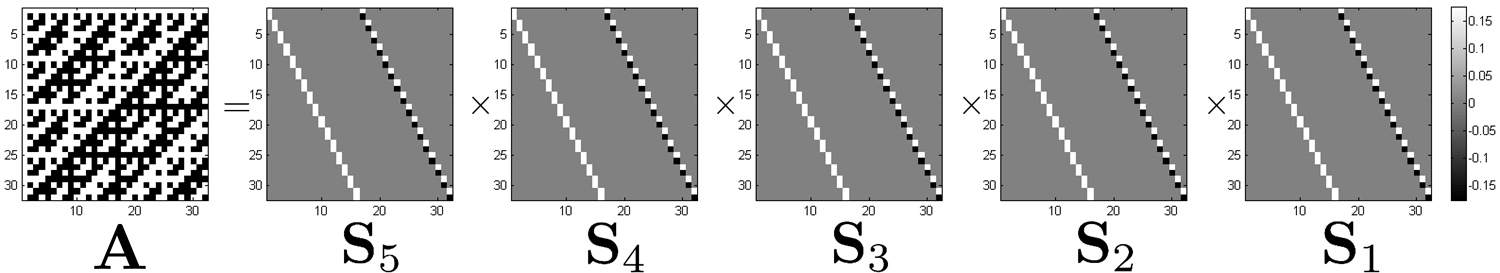
\includegraphics[scale=0.5]{images/hadamard32_bw.pdf}
\caption{Brief presentation of FA$\mu$ST}
\label{fig:presentation}
\end{figure}

FA$\mu$ST can be used to speed up iterative algorithms commonly used for solving high dimensional linear inverse problems. The algorithms implemented in the toolbox are described in details by Le Magoarou.\cite{LeMagoarou2016}.
The FA$\mu$ST toolbox is delivered with a Matlab wrapper. 
For more information on the FAuST project, please visit the website of the project: \url{http://faust.gforge.inria.fr}.

%\paragraph{Brief description:} 
%$A=\prod_{j=1}^J S_j$.


\paragraph{License:}Copyright (2016) Luc Le Magoarou, Remi Gribonval INRIA Rennes, FRANCE \\
The FAuST Toolbox is distributed under the terms of the GNU Affero General Public License. This program is free software: you can redistribute it and/or modify it under the terms of the GNU Affero General Public License as published by the Free Software Foundation. This program is distributed in the hope that it will be useful, but WITHOUT ANY WARRANTY; without even the implied warranty of MERCHANTABILITY or FITNESS FOR A PARTICULAR PURPOSE.  See the GNU Affero General Public License for more details. You should have received a copy of the GNU Affero General Public License along with this program.  If not, see \url{http://www.gnu.org/licenses/}.

\paragraph{FA$\mu$ST Structure:}
The Figure \ref{fig:faustStructure} presents a brief structure of the FA$\mu$ST toolbox. The principal C++ library called "libfaust" includes two components: the "Factorization algorithms" is used to generate a FA$\mu$ST matrix from a dense matrix and the "FA$\mu$ST matrix representation" provides a linear operator efficient for multiplication. It can be used from various types of environment. But currently (FA$\mu$ST package Version 2.0), only Matlab wrapper is provided. A Python wrapper is under development and should be available in the next version. 

\begin{figure}[H] %%[!htbp]
\centering
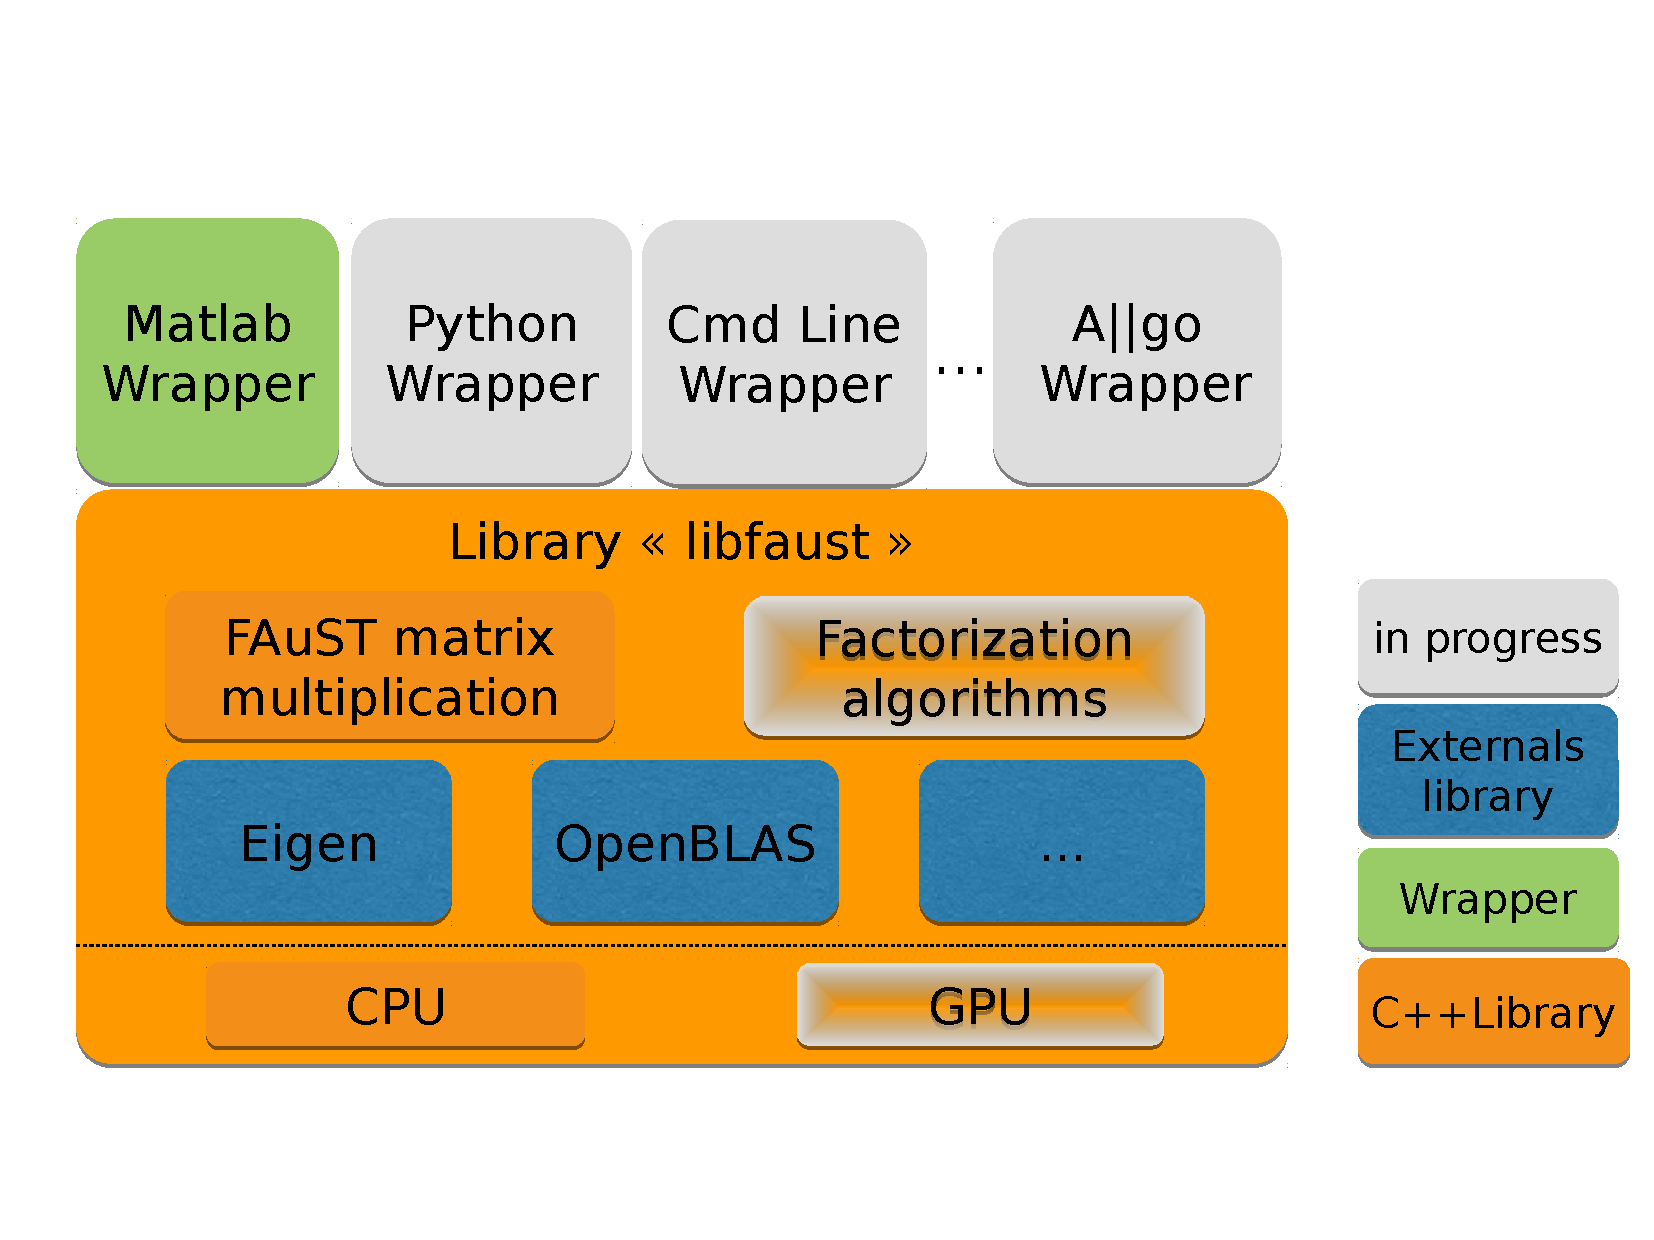
\includegraphics[scale=0.45,trim = 0cm 5cm 0cm 4cm, clip]{images/FaustStructure.pdf}
\caption{Brief structure of FAuST version 2.0.0}
\label{fig:faustStructure}
\end{figure}


\paragraph{Valid Installation: Platforms, Compiler and IDE}
The Figure \ref{fig:recapInstall} summarizes the tested configurations of the installation of the FA$\mu$ST toolbox following the type of platform (Linux, Mac or Windows), compiler, version of Matlab and the type of Integrate Development Environment (IDE).\\
Choose among this Figure \ref{fig:recapInstall} the adapted platform and IDE following your system and refer to the corresponding Install Chapter. 
The installation using the GCC compiler directly from a command terminal on Unix platforms is suggested because it is more simple and requires fewer externals components. 

The installation on Windows Platform using Visual Studio IDE has been tested but there are compilation problems depending of the version of your Windows and your Visual Studio. This install configuration is not guaranteed but you can try and report any problem and/or suggestion on install-list of FA$\mu$ST project on \url{http://lists.gforge.inria.fr/pipermail/faust-install/}. 

\begin{figure}[H] %%[!htbp]
\centering
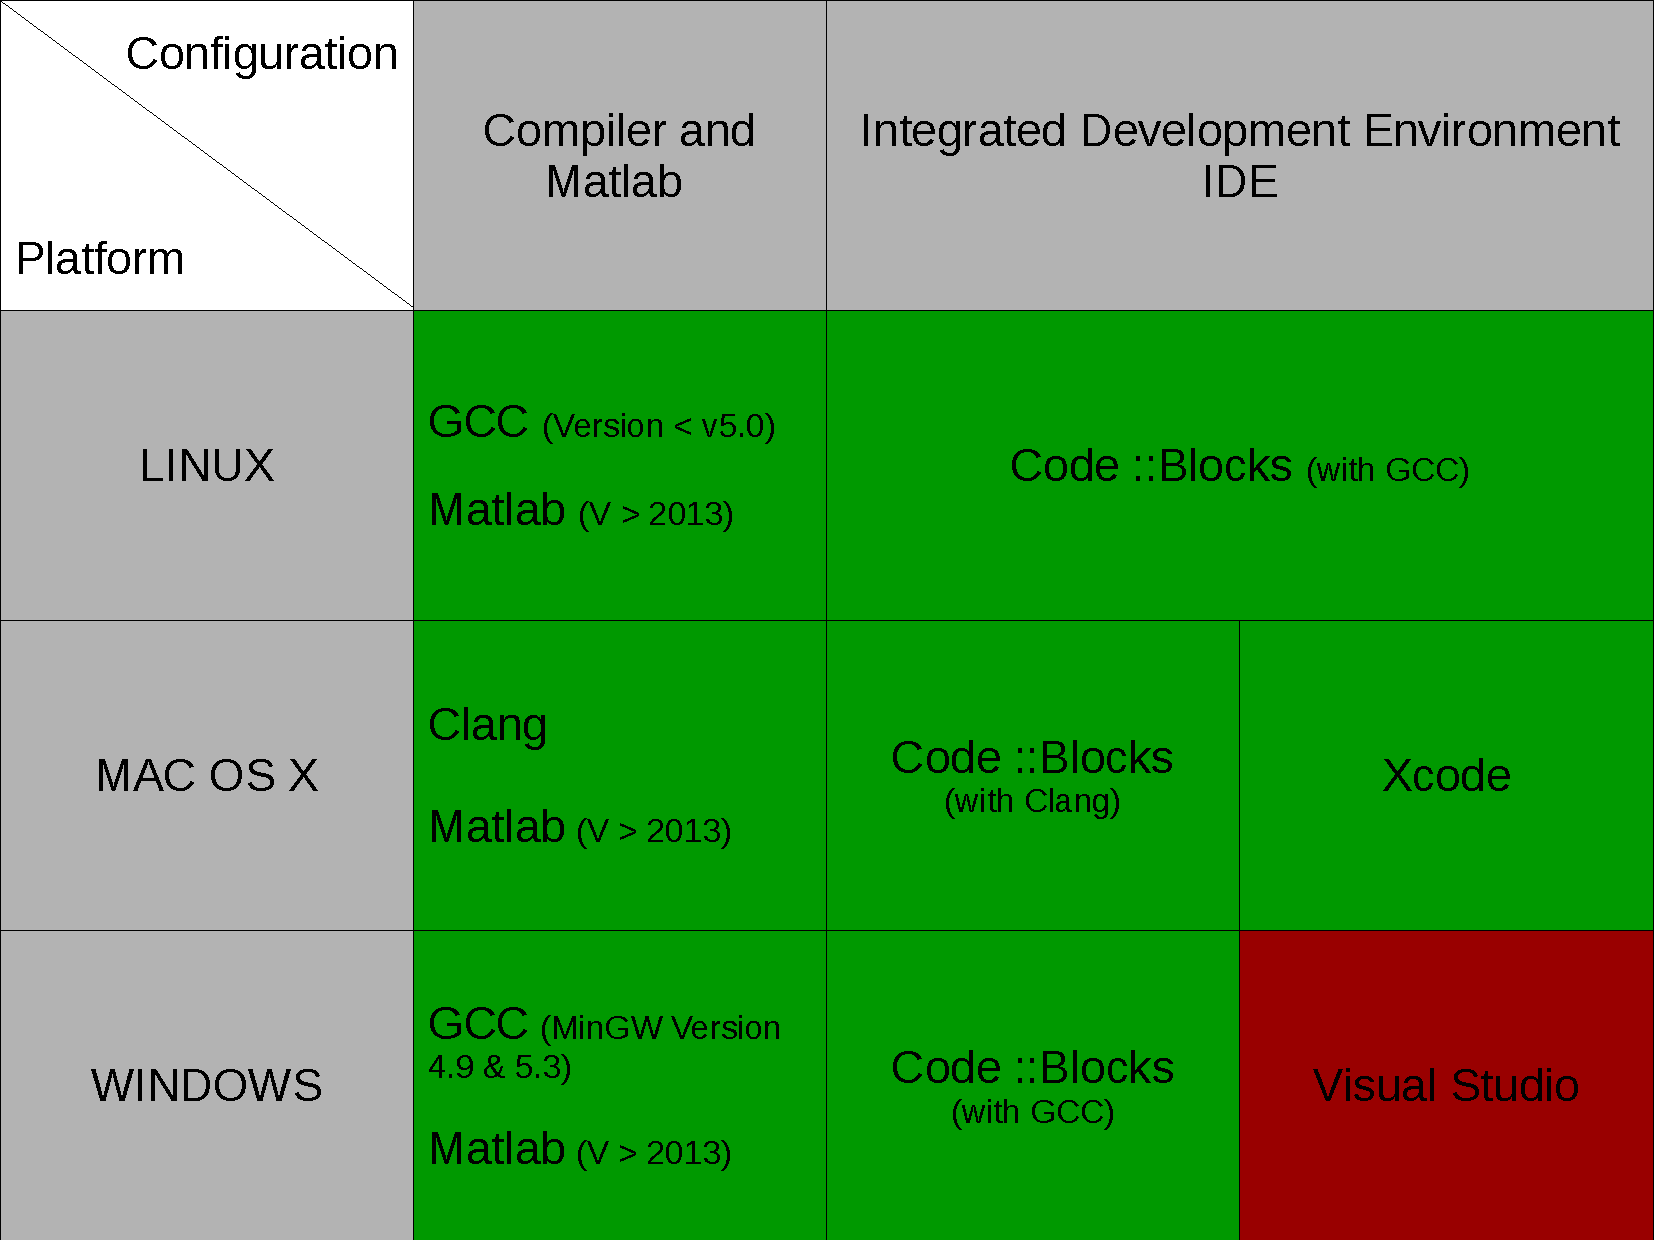
\includegraphics[scale=0.4]{images/recapInstall.pdf}
\caption{Checked Installation: Platforms and IDE}
\label{fig:recapInstall}
\end{figure}


\paragraph{Organization:}Chapter \ref{sec:InstallUnix} explains how to install the library FA$\mu$ST for UNIX platform and Chapter \ref{sec:WinInstall} corresponds to the Windows installation. Chapter \ref{sec:firstUse} shows quickly how to use this library and finally an example is given Chapter \ref{sec:example}. 

%!TEX root =  gettingStartedFAuST-version2_0.tex
\chapter{Installation on a Unix platform}\label{sec:InstallUnix}

The FA$\mu$ST project is available for Linux, MAC OS X and Windows platforms. The proposed toolbox provides a Matlab wrapper. \textbf{CMake} has been chosen to build the FA$\mu$ST project because it is an open-source, cross-platform family of tools designed to build, test and package software. This chapter presents the steps to install the FA$\mu$ST tools on a Unix platform (both Linux and Mac OS).

\begin{enumerate}
\item Ensure that the \textbf{prerequisite components} listed in Section \ref{sec:RequiredTools} are installed.

\item Refer to section \ref{sec:UnixBuildDownload} to download the FA$\mu$ST package and set your terminal. 

\item Refer to the appropriate section following the use (or not) of an IDE (Integrated Development Environment): 
\begin{itemize}
\item Basic installation using \textbf{the command line terminal}, refer to Section \ref{sec:UnixBuildInstall}.
\item Basic installation using \textbf{the Code::Blocks IDE}, refer to Section \ref{sec:UnixInstallCodeBlock}. 
\item Basic installation using \textbf{the Xcode IDE } only for MAC OS X platform, refer to Section \ref{sec:MacInstallXcode}. 
\end{itemize}
\end{enumerate}

Section \ref{sec:UnixCustomInstall} describes the custom options available to build the FA$\mu$ST toolbox, to propose a Custom - Advanced installation. For example, the optional configuration can be used to modify the install directory path, or to build in debug mode.  

Throughout the document we provide examples as follows:
\begin{itemize}
\item Command lines you must enter in a terminal are displayed as:
\lstset{style=customBash}
\begin{lstlisting}
> mkdir BUILD; ls . 
\end{lstlisting}
\item Messages resulting from such command lines appear without the leading '>':
\lstset{style=customBash}
\begin{lstlisting}
example of return text in your current terminal. 
\end{lstlisting}
\item Command lines you must enter in a Matlab Command Window are displayed as:
\lstset{style=customMatlab}
\begin{lstlisting}
>> y = A*x; 
\end{lstlisting}
\item Messages resulting from such command lines appear without the leading '>>':
\lstset{style=customMatlab}
\begin{lstlisting}
example of return text in Matlab Command Window. 
\end{lstlisting}
\end{itemize}


\section{Required components}\label{sec:RequiredTools}
This Section lists the required components you must install before to begin the FA$\mu$ST installation. 
\begin{itemize}
\item \textbf{Install CMake}. The minimum version required is Cmake version 3.0.2. Download binary distribution of CMake from their website \url{https://cmake.org/download/}.


\item \textbf{Verify Cmake install} by typing in a command terminal : 
\lstset{style=customBash}
\begin{lstlisting}
> which cmake
\end{lstlisting}
The command terminal returns the path of your Cmake binary file like

\begin{lstlisting}
/usr/bin/cmake
\end{lstlisting}
If not, add Cmake binary directory in the environment path. (in your ~/.bashrc file)

\item \textbf{Install Matlab} (minimal version required is Matlab 2014a \url{https://fr.mathworks.com/downloads/})

\item \textbf{Verify Matlab install} by typing in a terminal the following command : 
\begin{lstlisting}
> which matlab
\end{lstlisting}
You must obtain the path of your matlab binary file like: 
\begin{lstlisting}
/usr/local/bin/matlab
\end{lstlisting}
If not, add \texttt{matlab} binary directory in your environment path (in your ~/.bashrc file). 
\item \textbf{Verify Matlab} has a MEX supported compiler by typing in a Matlab Command Window :
\lstset{style=customMatlab}
\begin{lstlisting}
>> mex -setup C++
\end{lstlisting}

You must obtain this kind of message :
\begin{lstlisting}
MEX configured to use <YOURCOMPILER>  for C++ language compilation.
\end{lstlisting}

But if you have an error message of the style :
\begin{lstlisting}[moredelim={**[is][\color{blue}]{@}{@}},moredelim={[is][\underbar]{_}{_}}]
No supported compiler or SDK was found. For options, visit 
@_http:www.matworks.com/support/compilers/R<20XXx>/<ARCH>.html_@
\end{lstlisting}
Visit the webpage specified in the error message,
in order to see the list of compiler supported by your Matlab version \texttt{R<20XXx>} on your plateform \texttt{<ARCH>}.

\end{itemize}


\section{Download FAuST Package \& launch terminal}\label{sec:UnixBuildDownload}

When prerequisities listed in precedent section \ref{sec:RequiredTools} are checked, you can get the package FA$\mu$ST.
\begin{itemize}
\item \textbf{Download} the FA$\mu$ST package on the website :  \url{http://faust.gforge.inria.fr/}
\item \textbf{Unzip} the FA$\mu$ST package into your FA$\mu$ST directory.
\item \textbf{Open} a command terminal
\item \textbf{Set the current directory} to your FA$\mu$ST directory (NOTE: do not use any special character in your FA$\mu$ST directory path, for example the character $\mu$)
\end{itemize}



\section{Basic Build \& Installation using Makefile}\label{sec:UnixBuildInstall}

When you have done the step in section \ref{sec:UnixBuildDownload} (i.e download FA$\mu$ST package and launch the terminal in the right directory),  the FA$\mu$ST installation can start.
If you are administrator of your machine (root access), follow instructions given in Section \ref{sec:UnixBuildInstallAdmin}. Otherwise, for local installation, refer to Section \ref{sec:UnixBuildInstallNOAdmin}. 

\subsection{Install with administrator privilege}\label{sec:UnixBuildInstallAdmin}
In the terminal opened in Section 
\ref{sec:UnixBuildDownload}, type the following commands : 
\lstset{style=customBash}
\begin{lstlisting}
> mkdir build
> cd build
> cmake ..
> make
> sudo make install # run with administrator privilege
\end{lstlisting}

FA$\mu$ST Toolbox should be installed. Now, refer to Quick-Start Chapter \ref{sec:firstUse} to check the install and to try FA$\mu$ST toolbox.

For more detail about \texttt{cmake ; make ; make install} commands, refer to Section \ref{sec:ANNEXEInfoBuildInstall}.


\subsection{Install without administrator privilege}\label{sec:UnixBuildInstallNOAdmin}
In the terminal opened in Section \ref{sec:UnixBuildDownload}, type the following commands :
\lstset{style=customBash}
\begin{lstlisting}
> mkdir build
> cd build
> cmake .. -DCMAKE_INSTALL_PREFIX="<Your/Install/Dir>"
> make
> make install
\end{lstlisting}

FA$\mu$ST Toolbox should be installed. Now, refer to Quick-Start Chapter \ref{sec:firstUse} to check the install and to try FA$\mu$ST toolbox.

For more detail about \texttt{cmake ; make ; make install} commands, refer to Section \ref{sec:ANNEXEInfoBuildInstall}.


% CODEBLOCKS
\section{Basic Build \& Install using Code Block IDE}\label{sec:UnixInstallCodeBlock}
When you have done the step in section  \ref{sec:UnixBuildDownload} (i.e download FA$\mu$ST package and launch the terminal in the right directory),  the FA$\mu$ST installation can start. If you are administrator of your machine (root access), follow instructions given in Section \ref{sec:CodeBlocUnixBuildInstallAdmin}. Otherwise, for local installation, refer to Section \ref{sec:CodeBlocUnixBuildInstallNOAdmin}. 

\subsection{Install with administrator privilege}\label{sec:CodeBlocUnixBuildInstallAdmin}
\begin{itemize}
\item In the terminal opened in section 
\ref{sec:UnixBuildDownload}, type the following commands : 
\lstset{style=customBash}
\begin{lstlisting}
> mkdir build
> cd build
> cmake .. -G "CodeBlocks - Unix Makefiles"
\end{lstlisting}

\item Open the FA$\mu$ST project from the file \textbf{./build/FAUST.cbp} with Code::Blocks IDE. 
\item In Code::Blocks IDE, select \textbf{ALL} target and build the project. 
\item Close Code::Blocks IDE
\item Re-Open the FA$\mu$ST project from the file \textbf{./build/FAUST.cbp} with Code::Blocks IDE \textbf{with administrator privilege}. For that, type in a terminal :
\begin{lstlisting}
> sudo codeblocks
\end{lstlisting}
\item In Code::Blocks IDE, select \textbf{install} target and build the project. 
\end{itemize}

FA$\mu$ST Toolbox should be installed. Now, refer to Quick-Start Chapter \ref{sec:firstUse} to check the install and to try FA$\mu$ST toolbox.

For more detail about \texttt{cmake} command, refer to Section \ref{sec:ANNEXEInfoBuildInstall}.


\subsection{Install without administrator privilege}\label{sec:CodeBlocUnixBuildInstallNOAdmin}
\begin{itemize}
\item In the terminal opened in section 
\ref{sec:UnixBuildDownload}, type the following commands : 
\lstset{style=customBash}
\begin{lstlisting}
> mkdir build
> cd build
> cmake .. -G "CodeBlocks - Unix Makefiles"
  		   -DCMAKE_INSTALL_PREFIX="<Your/Install/Dir>"
\end{lstlisting}

\item Open the FA$\mu$ST project from the file \textbf{./build/FAUST.cbp} with Code::Blocks IDE. 
\item In Code::Blocks IDE, select \textbf{ALL} target and build the project. 
\item In Code::Blocks IDE, select \textbf{install} target and build the project. 
\end{itemize}

FA$\mu$ST Toolbox should be installed. Now, refer to Quick-Start Chapter \ref{sec:firstUse} to check the install and to try FA$\mu$ST toolbox.

For more detail about \texttt{cmake} command, refer to Section \ref{sec:ANNEXEInfoBuildInstall}.


% Xcode 
\section{Basic Build \& Install using Xcode IDE (for MAC OS)}\label{sec:MacInstallXcode}

FA$\mu$ST install using the Xcode IDE concerns only MAC OS X environment.
\paragraph{}When you have done the step in section  \ref{sec:UnixBuildDownload} (i.e download FA$\mu$ST package and launch the terminal in the right directory),  the FA$\mu$ST installation can start. This Build \& Install section requires that you have the Xcode IDE installed on your system. If you are administrator of your machine (root access), follow instructions given in Section \ref{sec:XcodeUnixBuildInstallAdmin}. Otherwise, for local installation, refer to Section \ref{sec:XcodeUnixBuildInstallNOAdmin}. 

\paragraph{NOTE: }For a command line install using Xcode IDE, refer to Annex \ref{sec:ANNEXEInstallMACXcodeTerminal}.  

\subsection{Install with administrator privilege}\label{sec:XcodeUnixBuildInstallAdmin}
 
\begin{itemize}
\item In the terminal opened in section 
\ref{sec:UnixBuildDownload}, type the following commands : 
\lstset{style=customBash}
\begin{lstlisting}
> mkdir build
> cd build
> cmake .. -G "Xcode"
\end{lstlisting}

\item Open the FA$\mu$ST project from the file \textbf{./build/FAUST.xcodeproj} with Xcode IDE. 
\item In Xcode IDE, select \textbf{ALL} target and build the project. 
\item Close Xcode IDE
\item Re-Open the FA$\mu$ST project from the file \textbf{./build/FAUST.xcodeproj} with Xcode IDE \textbf{with administrator privilege}. For that, type in a terminal:
\lstset{style=customBash}
\begin{lstlisting}
> sudo Xcode
\end{lstlisting}
\item In Xcode IDE, select \textbf{install} target and build the project. 
\end{itemize}

FA$\mu$ST Toolbox should be installed. Now, refer to Quick-Start Chapter \ref{sec:firstUse} to check the install and to try FA$\mu$ST toolbox.

For more detail about \texttt{cmake} command, refer to Section \ref{sec:ANNEXEInfoBuildInstall}.


\subsection{Install without administrator privilege}\label{sec:XcodeUnixBuildInstallNOAdmin}
 
\begin{itemize}

\item In the terminal opened in section 
\ref{sec:UnixBuildDownload}, type the following commands : 
\lstset{style=customBash}
\begin{lstlisting}
> mkdir build
> cd build
> cmake .. -G "Xcode" 
		   -DCMAKE_INSTALL_PREFIX="<Your/Install/Dir>"
\end{lstlisting}

\item Open the FA$\mu$ST project from the file \textbf{./build/FAUST.xcodeproj} with Xcode IDE. 
\item In Xcode IDE, select \textbf{ALL} target and build the project. 
\item In Xcode IDE, select \textbf{install} target and build the project. 
\end{itemize}

FA$\mu$ST Toolbox should be installed. Now, refer to Quick-Start Chapter \ref{sec:firstUse} to check the install and to try FA$\mu$ST toolbox.

For more detail about \texttt{cmake} command, refer to Section \ref{sec:ANNEXEInfoBuildInstall}.

%\paragraph{NOTE:}You can generated the target using the terminal command \texttt{xcodebuild} :
%\begin{lstlisting}
%> mkdir build
%> cd build
%> cmake .. -G "Xcode"
%%% list all target of the project
%> xcodebuild -list -project FAUST.xcodeproj 
%%% Build the targets
%> xcodebuild -configuration "Release" -target "ALL_BUILD" build 
%%% performs the "make install"
%> xcodebuild -configuration "Release" -target "install" build 
%\end{lstlisting}


\section{Custom - Advanced Installation}\label{sec:UnixCustomInstall}

The project FA$\mu$ST can be configured with optional parameters, for example if you want to install FA$\mu$ST library in a different folder or to enable the parallel computing using multithread capacities provided by the OS. This build system can be parametrized using the Cmake Graphical User Interface, or the Cmake command line tools. 

The Cmake Graphical User Interface \texttt{ccmake} allows you to select option input. Set your current directory to your build directory and type in a terminal :
\lstset{style=customBash}
\begin{lstlisting}
> ccmake ..
\end{lstlisting}

The Cmake GUI appears in the console (see fig. \ref{fig:ccmake}). 

\begin{figure}[H] %%[!htbp]
\centering
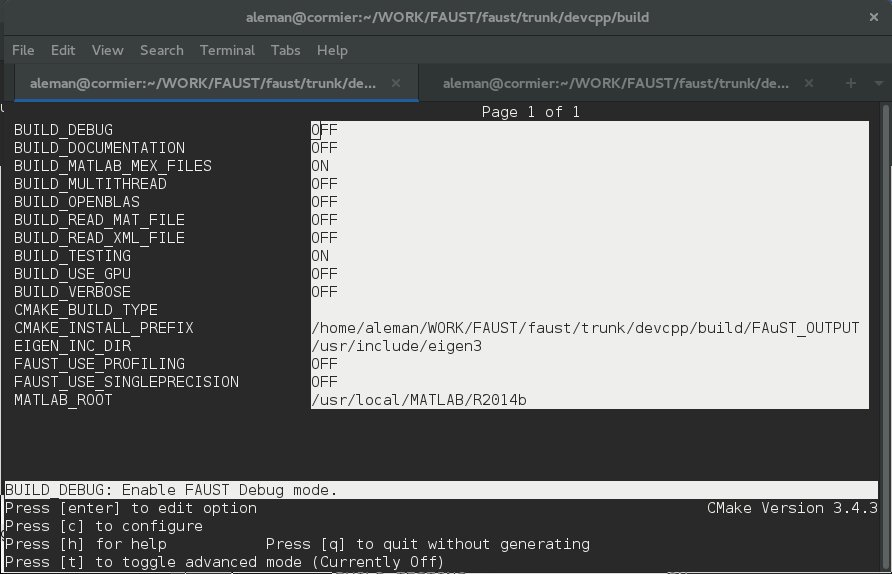
\includegraphics[scale=0.5]{images/ccmake.jpg}
\caption{ccmake GUI}
\label{fig:ccmake}
\end{figure}

When scrolling on a value and pressing [enter], this value can be edited, the black underlaid row displays some information about the option and required path to create the build system. In the case of an option press [enter] to toggle the ON/OFF values. You can edit option by pressing [enter]. For example, press [enter] to edit option \texttt{CMAKE\_INSTALL\_PREFIX} to modify the install directory. 

After choosing options for the build and setting the required fields, press [c] to configure. The configuration of the build system is checked again by Cmake, at the end of this check if the build settings are correct, you can press [g] in order to generate the build system.

Instead the ccmake GUI, an other possibility to configure and generate the project is to use the command line cmake which can take the option input. Here is the list of available options: 
\texttt{cmake\ ..\ -D<BUILD\_NAME>=<value>}

\begin{itemize}
\item CMAKE\_INSTALL\_PREFIX : Install directory path for the FA$\mu$ST library
\item CMAKE\_INSTALL\_MATLAB\_PREFIX : Install directory path for the Matlab wrapper
\item BUILD\_TESTING : Enable the ctest option (default value is ON)
\item BUILD\_DOCUMENTATION : Generating the doxygen documentation (default value is OFF)  
\item BUILD\_MULTITHREAD : Enable multithread with OpenMP Multithreading (default value is OFF)
\item BUILD\_VERBOSE : Enable verbose option when compile (-v) (default value is OFF)
\item BUILD\_DEBUG : Enable FA$\mu$ST Debug mode (default value is OFF )
\item BUILD\_USE\_GPU : Using both CPU and GPU process (default value is OFF) (refer to Section \ref{sec:OptionalGPU} for installation and more detail)
\item BUILD\_MATLAB\_MEX\_FILES : Enable building Matlab MEX files (default value is ON)
\item BUILD\_OPENBLAS : Using openBLAS for matrix and vector computations (default value is OFF )
%\item BUILD\_READ\_XML\_FILE : Using xml2 library to read xml files (default value is OFF)
%\item BUILD\_READ\_MAT\_FILE : Using matio library to read mat files (default value is OFF)
\end{itemize}

Following the selected option, the cmake installer automatically checks the dependent component (library OpenBlas, eigen).  

%\section{Optional dependent tools}\label{sec:OptionalRequiredTools}

%\paragraph{Optional Install of GPU process}
%\begin{itemize}
%\item \textbf{Install} CUDA and the drivers for NVIDIA.
%\item \textbf{Verify install} of GPU tools by typing in a terminal : 
%\begin{lstlisting}
%> which nvcc
%\end{lstlisting}
%You must obtain the path of your \texttt{nvcc} compiler like 
%\begin{lstlisting}[backgroundcolor=\color{white}]
%/usr/local/cuda-7.5/bin/nvcc
%\end{lstlisting}
%If not, add \texttt{nvcc} directory in your environment path (in your ~/.bashrc file). 
%\end{itemize}



\chapter{Installation on Windows platform}\label{sec:WinInstall}

\paragraph{}The FA$\mu$ST project is based on an C++ library available for both UNIX and Windows environments. CMake has been choose to build the project FA$\mu$ST because it is an open-source, cross-platform family of tools designed to build, test and package software.

\paragraph{}This chapter presents the steps to install the FA$\mu$ST tools on the Windows platform. First section \ref{sec:WinGettingStarted} presents the basic installation of FA$\mu$ST and second section \ref{sec:WinCustomInstall} corresponds to the advanced  installation.


\section{Getting Started} \label{sec:WinGettingStarted}

\subsection{Required tools}\label{sec:WinRequired}
The installation of the FA$\mu$ST tools depends on other components to be installed in order to run properly. 
\begin{enumerate}

\item \textbf{Install CMake} for building the FA$\mu$ST tools. 
From \url{https://cmake.org/download/}, download Binary distributions correspond to your environment (in our case  cmake-3.6.1-win64-x64.zip). The directory of binary must be add to the environment PATH of your system if you want to use the cmake command line tool. 

% \item \textbf{Install 7-Zip} from \url{http://www.7-zip.org/}. 7-Zip is a file archiver used to extract external library files. Please verify that \texttt{7z.exe} is present in your environment PATH of your system.

\item \textbf{Install Matlab} if not already done (MATLAB R2015b in our case). The builder of the FA$\mu$ST tools automatically checks your Matlab root directory if your \texttt{matlab.exe} is present in your environment Path and/or if your Matlab installation has been performed in a default directory like \texttt{"C:/Program Files/MATLAB/<R2015b>/bin/matlab.exe"} or \texttt{"C:/Program Files (x86)/MATLAB/<R2015b>/bin/matlab.exe"}. In case of several versions of Matlab installed in your system, you can force the directory of your preferred version of Matlab using the following system variable : \\
\texttt{MATLAB\_EXE\_DIR="C:/Program Files/MATLAB/<R2015b>/bin/matlab.exe"}

\textit{Note for the case of using the compiler MinGW :} In Matlab, you must install MinGW version 4.9.2 from MATLAB using the \textbf{ADDON menu}. For more detail, please follow the instruction given in following link :  
\url{http://fr.mathworks.com/help/matlab/matlab_external/install-mingw-support-package.html}. For that, you must have a id session for Mathwork. It is easy to create. 
Current this latest step, an environment variable called MW\_MINGW64\_LOC is automatically generated. 

\item \textbf{Install C++ Compiler:} Both \textbf{Microsoft visual C++} and \textbf{MinGW "Minimalist GNU for Windows"} compiler have been tested. If you are friendly with Unix tools and command line terminal, preferd \textbf{MinGW "Minimalist GNU for Windows"} C++ compiler. Otherwise, if you are more familiar with the graphical user interface, prefer the \textbf{Microsoft visual C++} compiler. The version of the C++ compiler must be coherent with the version of your Matlab version. In this documentation, the version of our C++ compiler corresponds to Matlab 2014 and 2015. If you use an other version of Matlab, please refer to the Mathworks website \url{http://fr.mathworks.com/support/compilers/<R20XXa>}.

\paragraph{}For \textbf{Microsoft visual C++} installation :
\begin{itemize}
\item Download and install Microsoft Visual C++ 2013 professional from \url{https://www.microsoft.com/en-US/download/details.aspx?id=44916}
% \item Download and install Microsoft .NET Framework 4
% \item Download and install Microsoft SDK 7.1
\end{itemize}

\paragraph{}For \textbf{MinGW} installation :
\begin{itemize}
\item Download Mingw in \url{https://sourceforge.net/projects/mingw/files/latest/download?source=files}
\item Launch install file and choose MINGW version 4.9.2 for mexFunction compatibility 
\item The directory of binary must be add to the environment PATH. 

\item \textit{Note for make tool :} In a terminal command, type \texttt{make}. if it doesn't exist, please check if \textbf{make.exe} file is present in MINGW install directory. if not, you can copy and rename mingw32-make.exe to make.exe
\end{itemize}

\end{enumerate}


\subsection{Required packages}\label{sec:WinRequiredPackages}
\paragraph{}Here is a list of packages used in the FA$\mu$ST project. There are nothing to do because the installation of this packages are automatically done (see the directory "./externals").
\begin{itemize}
\item \textbf{Eigen} is a C++ template library for linear algebra: matrices, vectors, numerical solvers, and related algorithms. (see \url{http://eigen.tuxfamily.org})

\end{itemize}


\subsection{Basic build and Installation}\label{sec:WinBasicInstall}
\paragraph{}When prerequisites listed in previous section \ref{sec:WinRequired} are checked, the FA$\mu$ST installation can be done. 
First download the FA$\mu$ST package on the website  \url{http://faust.gforge.inria.fr/}. 

Depending to your C++ compiler (MinGW or Visual studio), refer to the right part and follow the given instructions.
\\

\subsubsection{Using MinGW compiler:}
\label{sec:WinMinGWBasicInstall}

\begin{itemize}
\item Open a command terminal
\item Place you in your local FA$\mu$ST directory (NOTE: don't use any special character in your FAUST directory path, for example the character $\mu$)
\item Type the following commands : 

\begin{lstlisting}
mkdir build
cd build
cmake -G "MinGW Makefiles" .. 
make
make install % run with administrator privilege
\end{lstlisting}
\paragraph{NOTE:} You can generated the CodeBlocks project with the following command : \\
\texttt cmake -G "CodeBlocks - MinGW Makefiles" .. 

\end{itemize}

\subsubsection{Using Visual Studio compiler:}\label{sec:WinVisualStudioBasicInstall}
\paragraph{}In the case of \textbf{Microsoft Visual Studio 2013 compiler using the Graphical Users Interfaces}:
\begin{enumerate}
\item Open application \texttt{cmake-GUI.exe} from the program menu or from your cmake install binaries directory  to launch the CMake configuration application:

\begin{figure}[!h] %%[!htbp]
\centering
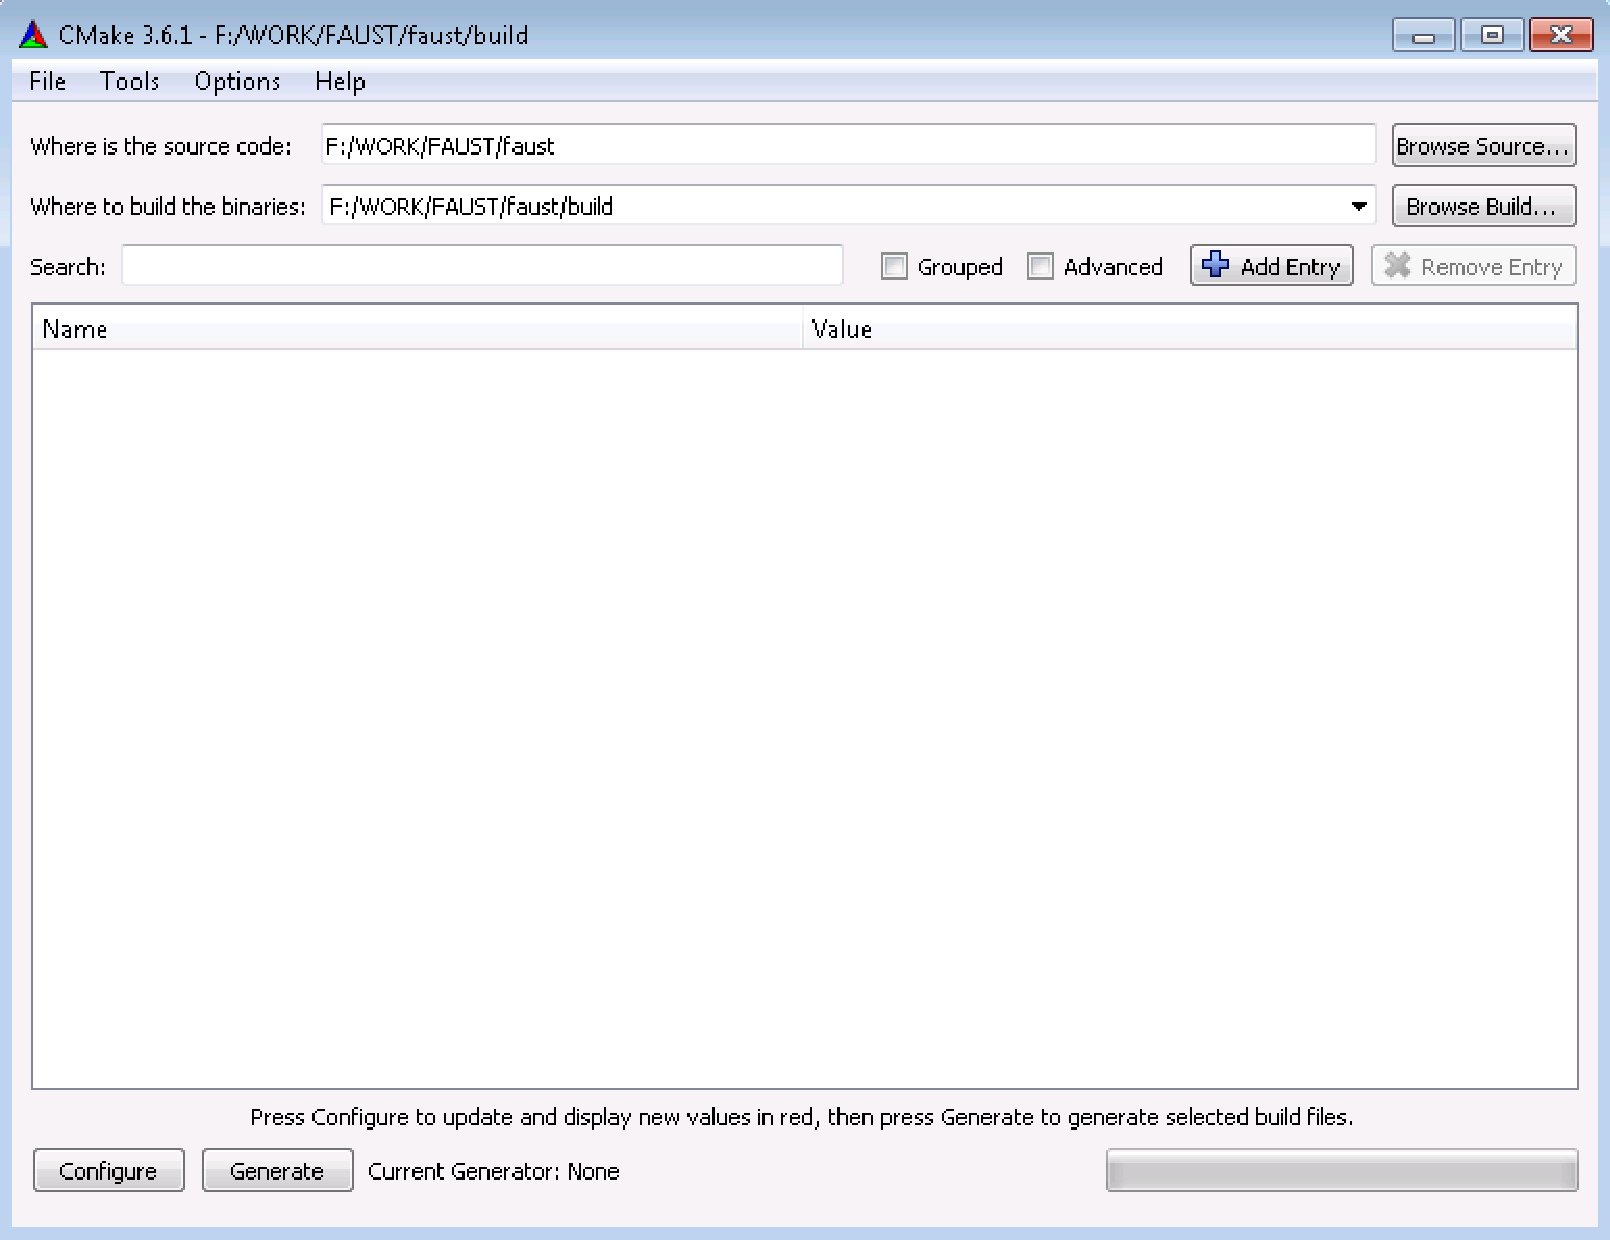
\includegraphics[scale=0.5]{images/cmakeGUI-1-eps-converted-to.pdf}
\caption{cmake GUI}
\label{fig:cmakeGUI-1}
\end{figure}

\item Set the "Where is the source code:" text box with the path of the directory where the source files are located (F:/WORK/FAUST/faust) and the "Where to build the binaries:" with the path of the directory where you want to build the library and executable files (F:/WORK/FAUST/faust/build). (see fig.  \ref{fig:cmakeGUI-1}).

When clicking for the first time on the [Configure] button, CMake will ask for the build tool you want to use. The build system type depends on the builder you want to use, in our case this is the Visual Studio X (X depending the version of Visual installed on the computer) chain tools. (see fig. \ref{fig:cmakeGUI-2}).


\begin{figure}[!h]
\centering
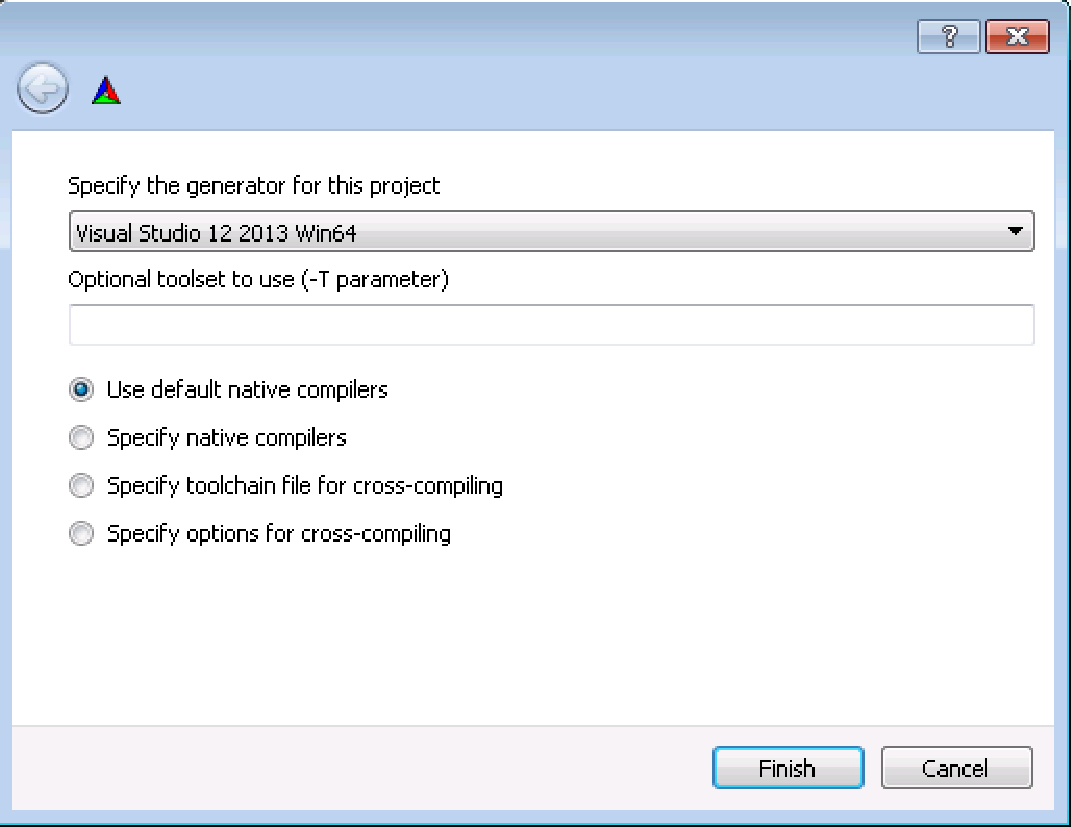
\includegraphics[scale=0.5]{images/cmakeGUI-2-eps-converted-to.pdf}
\caption{cmake GUI}
\label{fig:cmakeGUI-2}
\end{figure}

\item When pressing again the [Configure] button to configure the build system, CMake performs a list of tests to determine the system configuration and manage the build system. If the configuration is correct then no pop-up will appears during the tests and CMake finally shows the various options of the build underlaid in grey. In case of a configuration issue, a pop up window warns you about this issue indicating which test has failed, in this case the build option in the CMake application software will be underlaid in red. We will discuss in Section \ref{sec:WinCustomInstall} what to do in such a case, but let us for the moment assume that everything ran smoothly.
(see \ref{fig:cmakeGUI-4}).

\begin{figure}[!h] %%[!htbp]
\centering
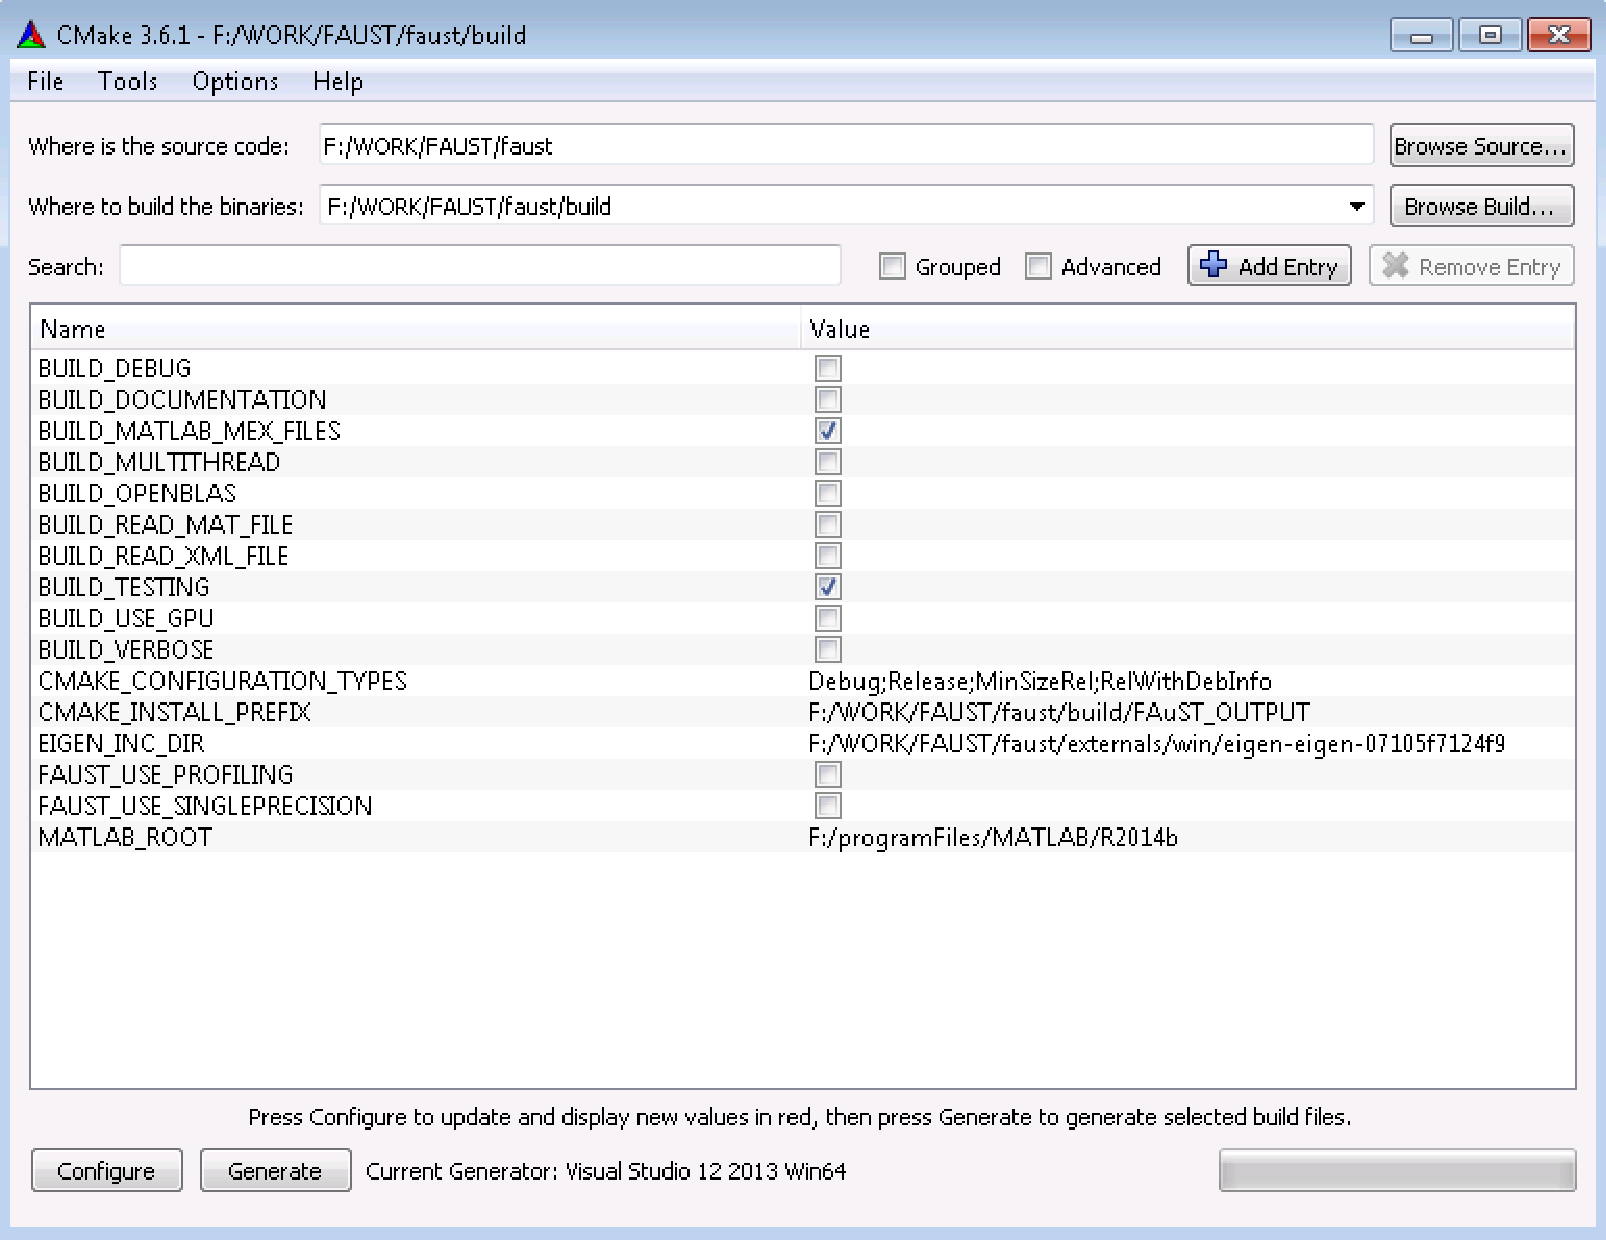
\includegraphics[scale=0.5]{images/cmakeGUI-4-eps-converted-to.pdf}
\caption{cmake GUI}
\label{fig:cmakeGUI-4}
\end{figure}

\item Once the build system configured then generated, you have to actually build FAUST, using Visual Studio.
\item Open file "faust.sln" with visual studio 
\item Click right on Target ALL\_BUILD and select generated 
\item Click right on Target INSTALL and select generated 
\item Click right on Target CTEST and select generated 
\end{enumerate}



\paragraph{}In the case of \textbf{Microsoft Visual Studio 2013 compiler using the command terminal} :

\begin{itemize}
\item Open a command terminal
\item Place you in your local FA$\mu$ST directory (NOTE: don't use any special character in your FAUST directory path, for example the character $\mu$)
\item Type the following commands : 

\begin{lstlisting}
mkdir build
cd build
cmake .. 
cmake --build . --config "Release" --target "install"
\end{lstlisting}

\end{itemize}

\section{Custom - Advanced Installation}\label{sec:WinCustomInstall}

progress... 




\chapter{QuickStart}\label{sec:firstUse}


\paragraph{}A Matlab wrapper is delivered with the FA$\mu$ST C++ library.
It provides a user friendly new class of matrix \textbf{Faust} efficient for the multiplication with matlab built-in dense matrix class.\newline

\section{Configure Matlab path}\label{sec:firstUseMatlabPath}
In order to use matlab wrapper after the installation of Faust, launch Matlab.
In the Matlab terminal, set your working directory to /"HOMEDIR"/Documents/MATLAB/Faust and configure the Matlab path by typing the following commands :

\begin{lstlisting}
>> cd /"HOMEDIR"/Documents/MATLAB/Faust
>> setup_Faust
\end{lstlisting}



\section{Use a faust from a saved one}\label{sec:firstUseBuildFromSave}
\paragraph{} Now, you can run quick\_start.m script in the Matlab terminal by typing :
\begin{lstlisting}
>> quick_start
\end{lstlisting}
\paragraph{}In this script, first of all, a Faust of size 4000x5000 is loaded from a previous one that is saved into a matfile :
\lstinputlisting[firstline=47,lastline=48,backgroundcolor=\color{white}]{../../misc/demo/Quick_start/quick_start.m}
\newpage
\paragraph{}Secondly, a list of overloaded matlab function shows that a Faust is handled as a normal Matlab builtin matrix.
 
\lstinputlisting[firstline=51,lastline=78,backgroundcolor=\color{white}]{../../misc/demo/Quick_start/quick_start.m}

\paragraph{}Finally, it performs a little time comparison between multiplication by a Faust or its full matrix equivalent.
This is in order to illustrate the speed-up induced by the Faust. This speed-up should be around 30 (depending on your machine).
%\lstinputlisting[firstline=84,lastline=100,backgroundcolor=\color{white}]{../../misc/demo/Quick_start/quick_start.m}

\newpage
\section{Construct a Faust from a given matrix}\label{sec:firstUseBuildFromMatrix}
\paragraph{} To see an example of building a Faust from a matrix, you can run factorise\_matrix.m in the Matlab terminal by typing :
\begin{lstlisting}
>> factorise_matrix
\end{lstlisting}
In this script, from a given matrix A of size 100x200 :
\lstinputlisting[firstline=42,lastline=47,backgroundcolor=\color{white}]{../../misc/demo/Quick_start/factorise_matrix.m}
We generate the parameters of the factorisation from :\newline
-the dimension of A (\textbf{dim1} and \textbf{dim2}),\newline
-\textbf{nb\_factor} the number of factor of the Faust,\newline
- and \textbf{rcg} the Rational Complexity Gain, which represents the theoretical memory gain and multiplication speed-up of the Faust compared to the initial matrix 
\lstinputlisting[firstline=51,lastline=56,backgroundcolor=\color{white}]{../../misc/demo/Quick_start/factorise_matrix.m}
Then we factorize the matrix \textbf{A} into a Faust \textbf{Faust\_A}
\lstinputlisting[firstline=58,lastline=59,backgroundcolor=\color{white}]{../../misc/demo/Quick_start/factorise_matrix.m}
And as for quickstart.m, we make some time comparison at the end.

\newpage
\section{Construct a Faust from its factor}\label{sec:firstUseBuildFactors}
To see an example of building a Faust from its factors, you can run construct\_Faust\_from\_factors.m in the Matlab terminal by typing :
\begin{lstlisting}
>> construct_Faust_from_factors
\end{lstlisting}
This following example shows how to build a faust from a cell-array representing its factors.
\lstinputlisting[firstline=44,lastline=72,backgroundcolor=\color{white}]{../../misc/demo/Quick_start/construct_Faust_from_factors.m}


 

\chapter{Example}\label{sec:example}

\section{Brain Sources Localization}\label{sec:BSL_example}
%\lstinputlisting{../../misc/demo/Brain_source_localization/BSL.m}



\paragraph{} An experience of Brain Source Localization using several gain matrices including FAuSTs and several solvers is provided. After configuring the matlab path (cf section \ref{sec:firstUseMatlabPath}). You can execute the matlab script \textbf{demo/Brain\_source\_localization/BSL.m} to run this experiment and \textbf{demo/Brain\_source\_localization/Fig\_BSL.m} to display the following pictures illustrating the speed-up using a Faµst.
You just need to type :
\begin{lstlisting}
>> BSL
>> Fig_BSL
\end{lstlisting}

Wich allows you to visualize this figure illustrating the speed-up with a Faust ($\mathbf{M}$ is the gain dense matrix and $\widehat{\mathbf{M}}_{6},\widehat{\mathbf{M}}_{9},\widehat{\mathbf{M}}_{16},\widehat{\mathbf{M}}_{26}$ are different Faust representing  $\mathbf{M}$):

\begin{figure}[!htbp]
\label{fig:BSL}
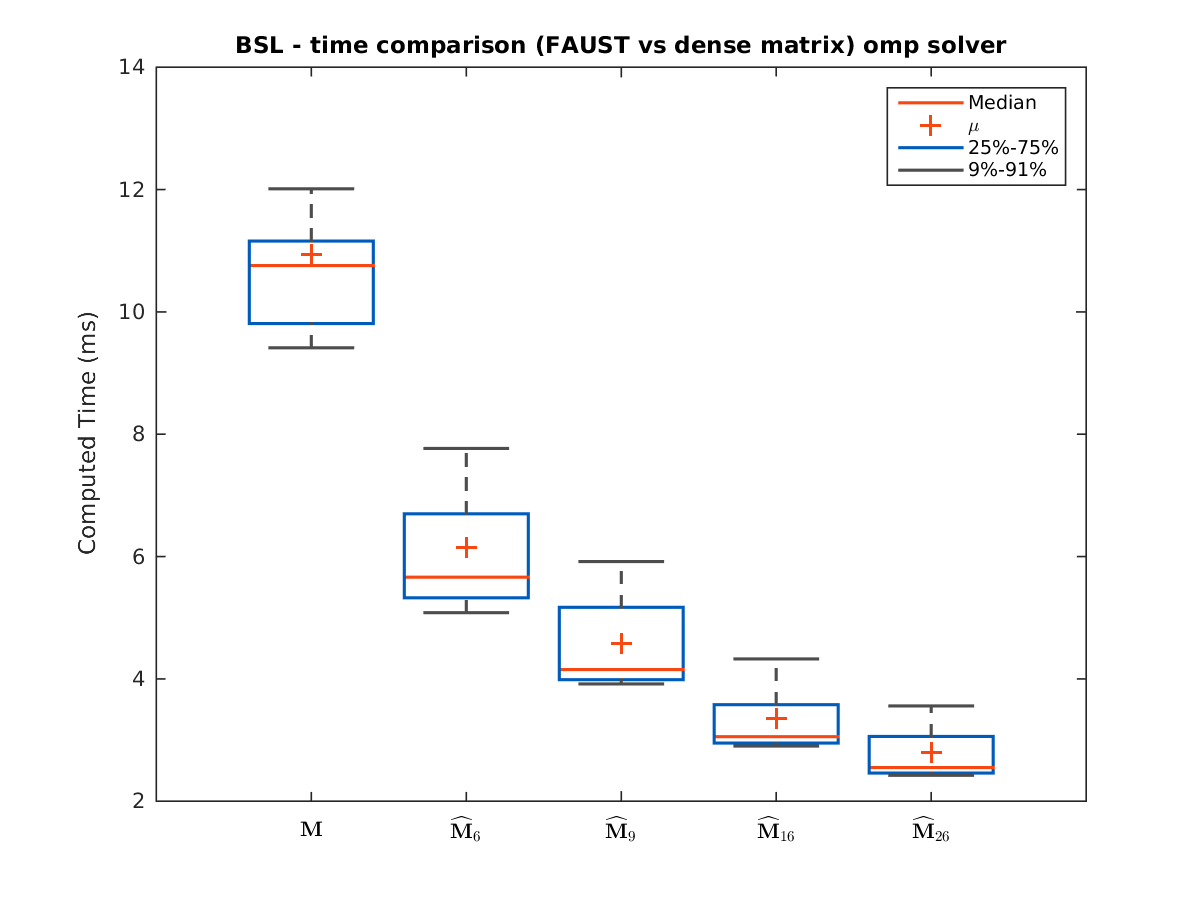
\includegraphics[scale=0.7]{images/BSL.png}
\end{figure}



\bibliographystyle{plain}
\bibliography{paperbiblio}


\end{document}



